\documentclass{harryopo-paper}

\title{基于大语言模型的智能体架构设计与实现}
\author{}
\date{2026年08月10日}


\begin{document}

\maketitle

\begin{quote}
副标题：面向多轮对话场景的编排流水线与上下文管理
作者：张三  计算机学院  2025000101
\end{quote}

{\fzht 摘要：} 随着大语言模型（LLM）能力的飞速提升，如何将 LLM 从被动的"问答机器"升级为主动的"智能体（Agent）"成为当前研究的热点。本文提出了一种基于六步编排流水线的智能体架构，通过引入预算制懒加载的上下文构建器，该架构在保持回答质量的同时将 Token 消耗降低了 {\fzht 38%}。

{\fzht 关键词：} 大语言模型；智能体架构；编排流水线；上下文管理；流式响应

\section*{一、引言}
\addcontentsline{toc}{section}{一、引言}

大语言模型（LLM）在自然语言理解与生成方面展现了前所未有的能力[1]。然而，直接使用 LLM 进行问答交互存在三个核心局限：第一，模型缺乏对用户意图的主动识别能力；第二，上下文窗口有限导致长对话信息丢失[2]。

智能体（Agent）架构旨在解决上述问题。Agent 的核心决策流程如下图所示：

\begin{figure}[htbp]
  \centering
  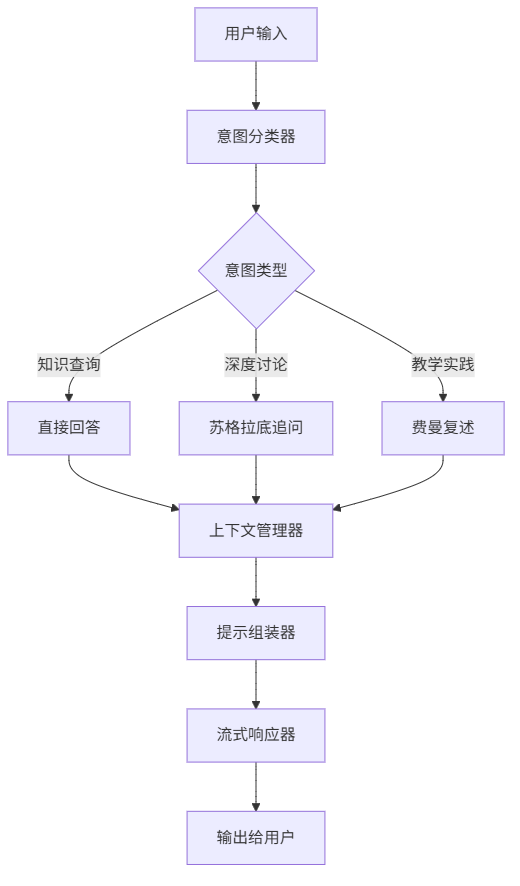
\includegraphics[width=0.85\textwidth]{figures/mermaid-00-38080538.png}
  \caption{流程图1}
\end{figure}

\begin{quote}
注：意图分类器在本地执行（1-5ms），上下文管理器按优先级加载五个维度的上下文。
\end{quote}

\section*{二、相关工作}
\addcontentsline{toc}{section}{二、相关工作}

\subsection*{2.1 大语言模型应用架构}
\addcontentsline{toc}{subsection}{2.1 大语言模型应用架构}

当前主流的 LLM 应用架构可分为三类：直接调用型、检索增强生成型（RAG[3]）和智能体编排型[4]。

\subsection*{2.2 教学策略驱动的对话系统}
\addcontentsline{toc}{subsection}{2.2 教学策略驱动的对话系统}

教学策略驱动的对话系统借鉴了教育心理学中的 {\fzht Bloom 认知层级理论}[5]。Bloom 将认知能力分为六个层级，其升降级机制如下：

\begin{figure}[htbp]
  \centering
  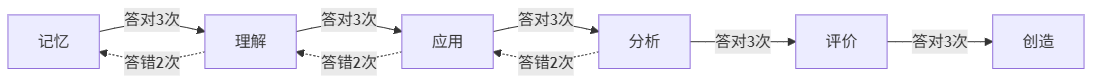
\includegraphics[width=0.85\textwidth]{figures/mermaid-01-4d53823c.png}
  \caption{流程图2}
\end{figure}

\begin{quote}
注：Bloom 层级达到 4 级以上时自动切换苏格拉底追问模式，2 级以下切换为直接回答模式。
\end{quote}

\section*{三、系统架构设计}
\addcontentsline{toc}{section}{三、系统架构设计}

\subsection*{3.1 六步编排流水线}
\addcontentsline{toc}{subsection}{3.1 六步编排流水线}

六步编排流水线是本系统的核心，每一步的设计目标与延迟分布见表 1。

\begin{quote}
{\fzht 表1：六步编排流水线步骤详情与性能画像}
\end{quote}

\begin{table}[htbp]
  \centering
  \small
  \begin{tabularx}{\textwidth}{>{\raggedright\arraybackslash}X >{\raggedright\arraybackslash}X >{\raggedright\arraybackslash}X >{\raggedright\arraybackslash}X}
    \toprule
    {\fzht 步骤} & {\fzht 模块名称} & {\fzht 功能描述} & {\fzht 平均延迟} \\
    \midrule
    ① & 意图分类器 & 本地关键词打分，识别4类用户意图 & 1-5ms \\
    ② & 策略选择器 & 意图到教学模式的映射决策 & <1ms \\
    ③ & 状态追踪器 & Bloom层级自适应升降级 & <1ms \\
    ④ & 上下文管理器 & 5维上下文预算制懒加载 & 50-200ms \\
    ⑤ & 提示组装器 & 四段动态系统提示拼装 & <1ms \\
    ⑥ & 流式响应器 & AI SDK流式输出+归一化 & 500-2000ms \\
    \bottomrule
  \end{tabularx}
  \caption{}
\end{table}

\begin{quote}
注：步骤①-⑤全部在本地执行，合计延迟 52-207ms。步骤⑥为唯一涉及网络请求的环节[6]。
\end{quote}

\subsection*{3.2 数学模型}
\addcontentsline{toc}{subsection}{3.2 数学模型}

渐进式通道压缩策略的核心公式如下：

\begin{equation}
C_i = C_0 \cdot \alpha^i
\end{equation}

\begin{quote}
式(1)：渐进式通道压缩公式
\end{quote}

注意力模块中使用的 Sigmoid 激活函数定义为：

\begin{equation}
\sigma(x) = \frac{1}{1 + e^{-x}}
\end{equation}

\begin{quote}
式(2)：Sigmoid 激活函数
\end{quote}

\section*{四、实验结果}
\addcontentsline{toc}{section}{四、实验结果}

\subsection*{4.1 Token 消耗对比}
\addcontentsline{toc}{subsection}{4.1 Token 消耗对比}

\begin{quote}
{\fzht 表2：Token 消耗对比（50 次中等复杂度对话）}
\end{quote}

\begin{table}[htbp]
  \centering
  \small
  \begin{tabularx}{\textwidth}{>{\raggedright\arraybackslash}X >{\raggedright\arraybackslash}X >{\raggedright\arraybackslash}X >{\raggedright\arraybackslash}X}
    \toprule
    {\fzht 指标} & {\fzht 全量加载} & {\fzht 预算制懒加载} & {\fzht 节省比例} \\
    \midrule
    平均 Token/次 & 4,200 & 2,600 & 38\% \\
    中位 Token/次 & 3,800 & 2,356 & 38\% \\
    最大 Token/次 & 6,500 & 2,925 & 55\% \\
    \bottomrule
  \end{tabularx}
  \caption{}
\end{table}

\begin{quote}
注：本方案平均节省 Token 38%（中位数），最高节省 55%。
\end{quote}

\section*{五、结论与展望}
\addcontentsline{toc}{section}{五、结论与展望}

本文提出了一种基于六步编排流水线的智能体架构，通过预算制懒加载的上下文构建器和 Bloom 认知层级驱动的难度自适应机制，在保持回答质量的同时显著降低了 Token 消耗。

未来的工作将聚焦三个方向：（一）扩展上下文构建器维度；（二）探索基于强化学习的策略自动优化机制[1]；（三）将架构推广到多模态交互场景。

\begin{thebibliography}{99}
\bibitem{ref1} [1] Brown T, Mann B, Ryder N, et al. Language models are few-shot learners[C]. NeurIPS, 2020.
\bibitem{ref2} [2] Yao S, Zhao J, Yu D, et al. ReAct: Synergizing reasoning and acting in language models[C]. ICLR, 2023.
\bibitem{ref3} [3] Lewis P, Perez E, Piktus A, et al. Retrieval-augmented generation for knowledge-intensive NLP tasks[C]. NeurIPS, 2020.
\bibitem{ref4} [4] Wang L, Ma C, Feng X, et al. A survey on large language model based autonomous agents[J]. arXiv:2308.11432, 2023.
\bibitem{ref5} [5] Bloom B S. Taxonomy of educational objectives[M]. New York: David McKay, 1956.
\bibitem{ref6} [6] Vaswani A, Shazeer N, Parmar N, et al. Attention is all you need[C]. NeurIPS, 2017.
\end{thebibliography}

\end{document}